\section{L'analyse des traces et la prononciation du verdict}
	L'analyse des traces et la prononciation des verdicts, est le c\oe{}ur de \textit{GreenT}, mais aussi une des parties les plus complexes. Comme expliqué précédemment, lors des stimulations un certain nombre de variables sont enregistrées, ensuite il faut évaluer l'\textit{Expected Behavior} à chaque instant T de la trace, qui est représenté au format CSV. 

	\subsection{Arbre de l'expectedBehavior}
 	Nous avons choisi de représenter l'\textit{Expected Behavior} sous la forme d'un arbre d'évaluation, cela nous permettra d'avoir plus de souplesse, en pouvant donner un verdict à une partie de l'arbre.

 	Chaque condition de l'\textit{Expected behavior} peut être transformée en une \textit{implication logique}, plusieurs evals à la suite correspondent à une conjonction logique de chacune des conditions des evals, et enfin, un else implique d'avoir eu la négation de la condition précédente. Figure \ref{fig:diagLogique}, nous pouvons voir un exemple d'\textit{Expected Behavior} et sa transformation en arbre.


L'\textit{Expected Behavior} contiendra des variables, celles-ci pourront être modifiées à tout moment ce qui relancera son évaluation, elle sera notifiée de cette modification à l'aide du patron de conception \textit{Observateur}. Une variable peut être spécifique en fonction du type de la variable, ceci afin d'aider les conversions.

 	\begin{figure}[H]
 		\centering
 		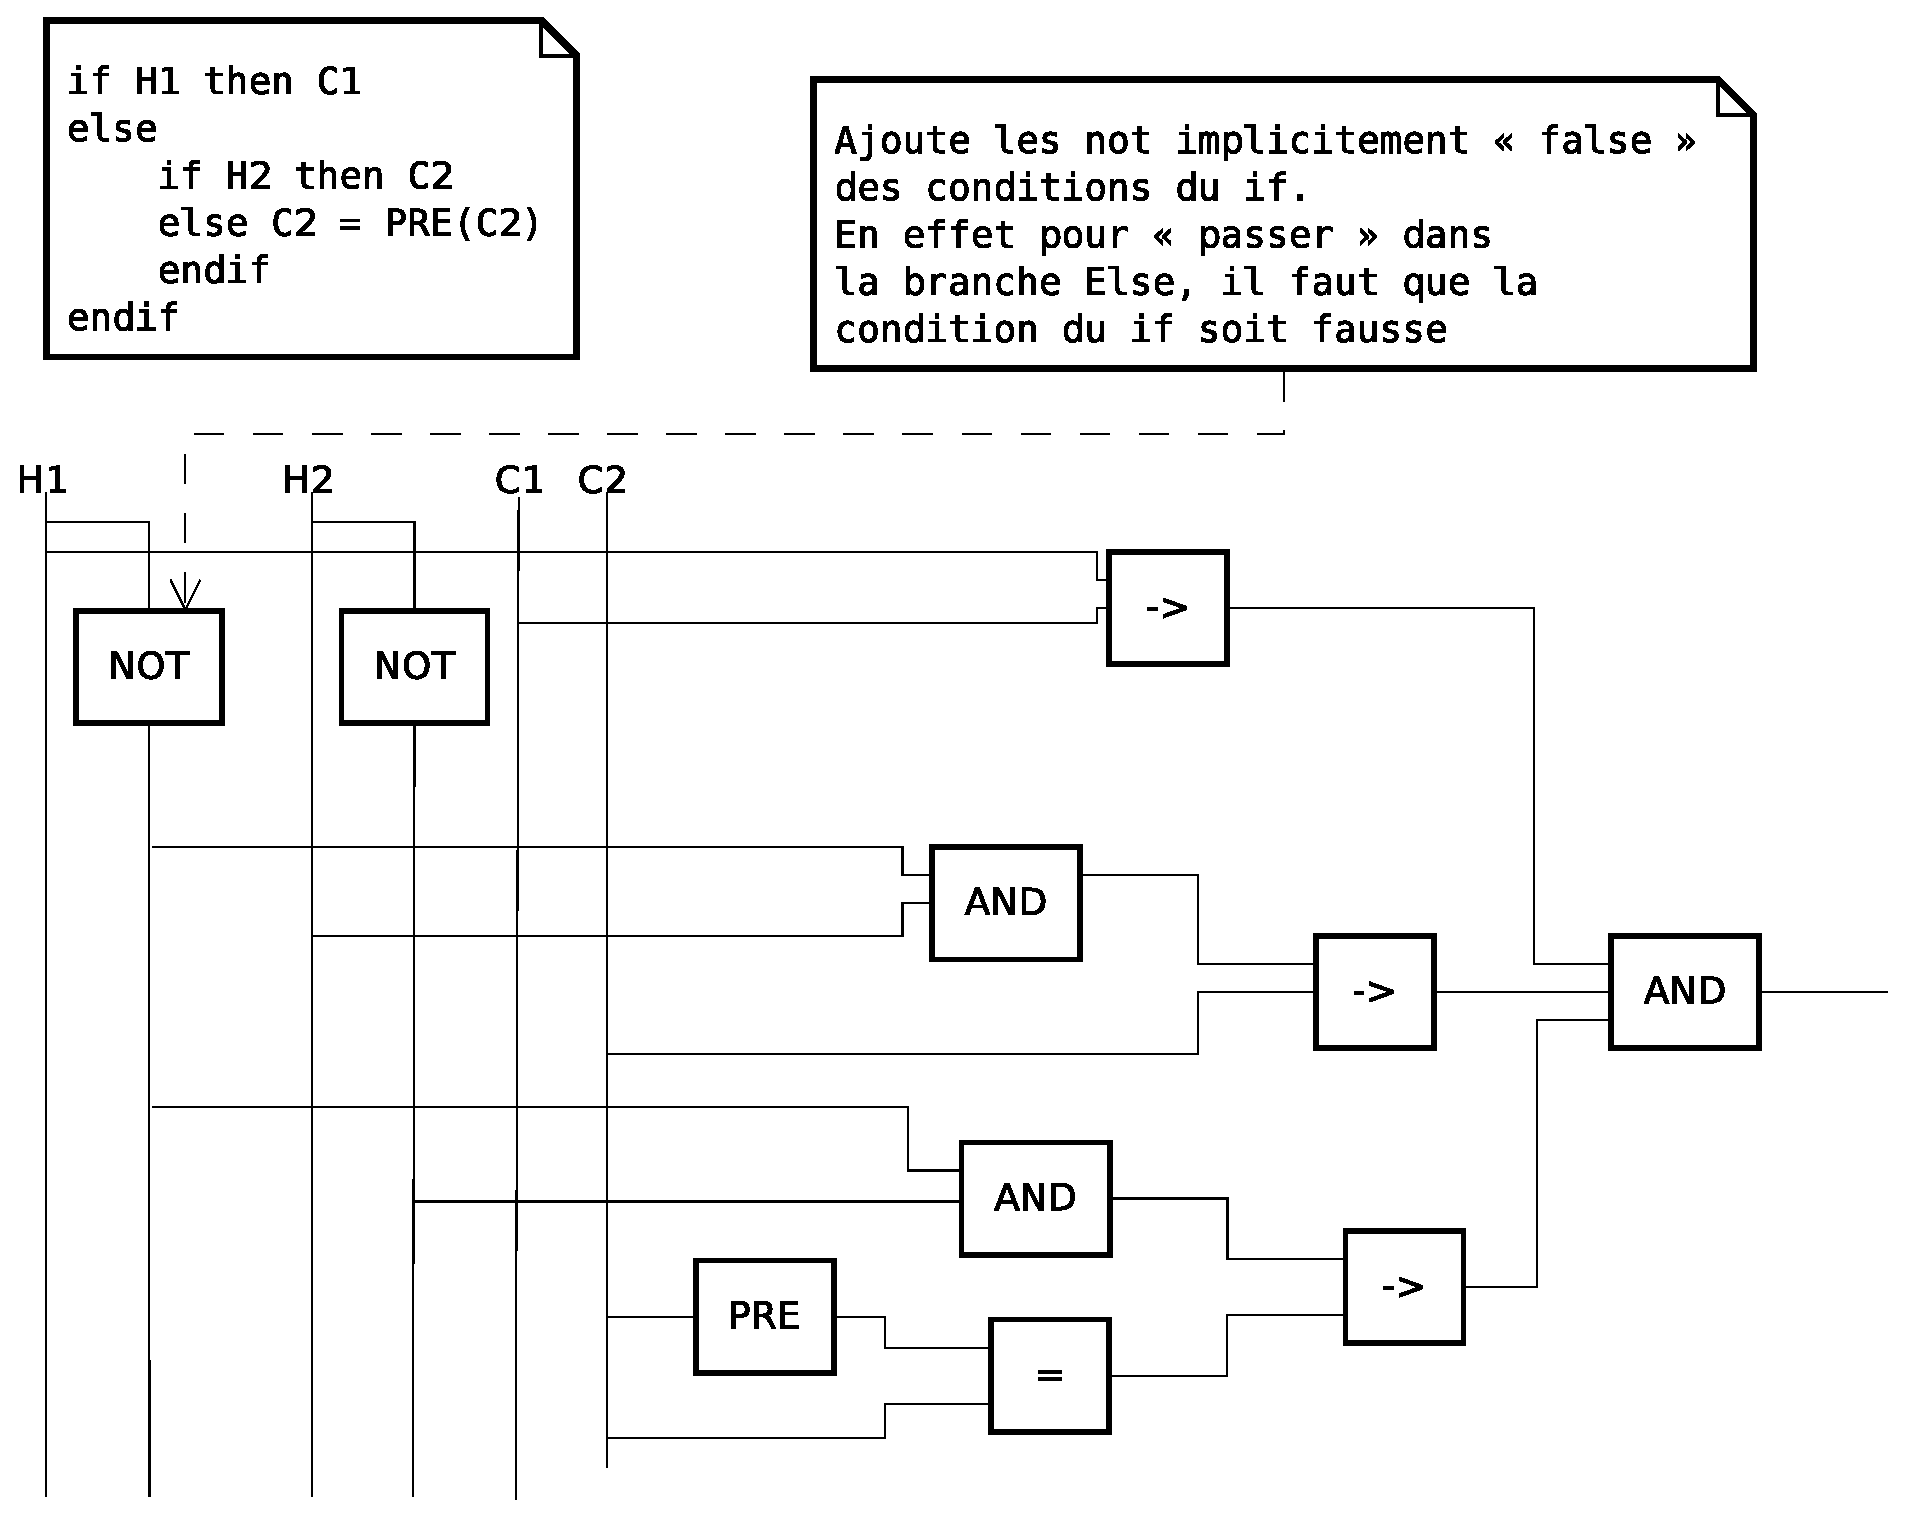
\includegraphics[width=14cm]{contents/images/diagLogique.eps}
 		\caption{Transformation d'une \textit{Expected Behavior} en arbre logique}
 		\label{fig:diagLogique}
 	\end{figure}

Une \textit{Expected Behavior} peut recevoir 3 états différents à l'issue de l'évaluation de la trace : 
\begin{description}
	\item[Rouge] Au moins un eval a renvoyé faux
	\item[Gris] Aucun eval n'a renvoyé faux, mais au moins une branche n'a pas été testée
	\item[Vert] Toutes les branches ont été testées, et tous les eval ont renvoyés vrais.
\end{description}

	\subsection{Analyse de la trace}
	Le fichier de trace au format CSV va être transformé en un dictionnaire ayant pour clé le timestamp et pour valeur la liste des variables ayant subi une
	modification, ainsi nous allons avoir une boucle itérant sur de dictionnaire qui à chaque itération modifiera les variables nécessaires, lors de cette modification
	une notification va être envoyée à l'\textit{Expected Behavior} qui relancera l'évaluation de la trace, le \texttt{TraceAnalyzer} stockera ce résultat dans le rapport. 

	De cette manière, il sera possible d'analyser l'\textit{Expected Behavior} à tout instant T de la trace.
	\vfill~\vfill

 	\begin{figure}[H]
 		\centering
 		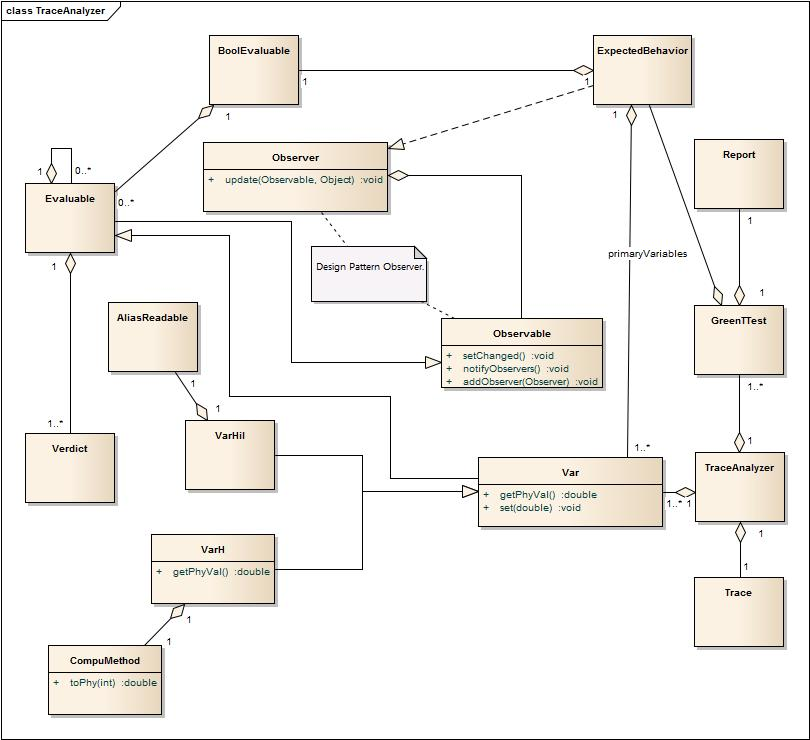
\includegraphics[width=17.5cm]{contents/images/TraceAnalyzer.jpg}
 		\caption{Diagramme de classe de l'analyse de trace}
 		\label{fig:diagLogique}
 	\end{figure}
 	Le n\oe{}ud racine de l'arbre d'expression sera un \texttt{BoolEvaluable} possédant un verdict(Rouge, Gris, Vert), et chaque n\oe{}ud de l'arbre et donc les \texttt{Variables} seront des \texttt{Evaluables}.
	\subsection{Prononciation du verdict}
	Chaque n\oe{}ud de l'arbre d'expression est susceptible d'avoir son propre verdict : ceci afin d'avoir plus de souplesse. Dans notre cas, seul les implications correspondant à une branche de \texttt{if...else} possèdera un verdict.
\vfill~\vfill

	\begin{figure}[H]
		\centering
		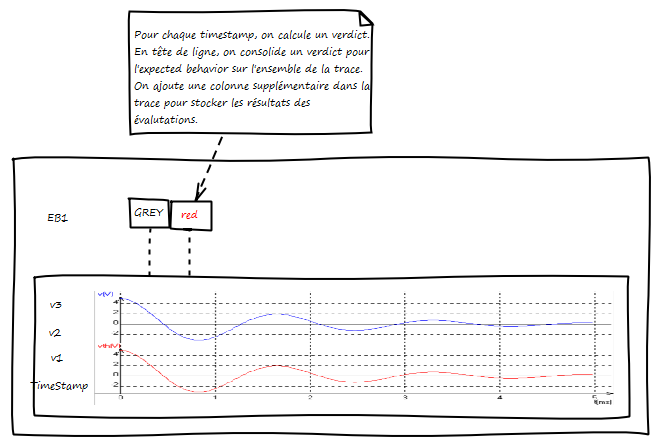
\includegraphics[width=16cm]{contents/images/trace.png}
		\caption{Exemple de Trace sous forme de courbes}
	\end{figure}

	\begin{remarque}
	À l'heure de l'écriture de ce rapport, cette partie n'a pas encore été implémentée, ayant 3 mois de stages, cela se fera durant le mois de stage supplémentaire.
	\end{remarque}
